\documentclass[UTF8]{ctexbeamer}
\usepackage{beamerthemesplit} % 加载主题宏包
\usetheme{Warsaw} % 选用该主题
\usepackage{subfig}
\usepackage{amsmath,amsthm,amssymb,amsfonts}
\usepackage{amsfonts,booktabs}
\usepackage{amsmath}
\usepackage{lmodern,textcomp}
\usepackage{color}
\usepackage{tikz}
\usepackage{natbib}
\usepackage{multicol}
\usepackage{caption}
\captionsetup[figure]{name={Figure}}
\usepackage{listings}
\usepackage{ctex}
\usepackage{pythonhighlight}
% 用来设置附录中代码的样式

\lstset{
	basicstyle          =   \sffamily,          % 基本代码风格
	keywordstyle        =   \bfseries,          % 关键字风格
	commentstyle        =   \rmfamily\itshape,  % 注释的风格,斜体
	stringstyle         =   \ttfamily,  % 字符串风格
	flexiblecolumns,                % 别问为什么,加上这个
	numbers             =   left,   % 行号的位置在左边
	showspaces          =   false,  % 是否显示空格,显示了有点乱,所以不现实了
	numberstyle         =   \zihao{-5}\ttfamily,    % 行号的样式,小五号,tt等宽字体
	showstringspaces    =   false,
	captionpos          =   t,      % 这段代码的名字所呈现的位置,t指的是top上面
	frame               =   lrtb,   % 显示边框
}

\lstdefinestyle{Python}{
	language        =   Python, % 语言选Python
	basicstyle      =   \zihao{-5}\ttfamily,
	numberstyle     =   \zihao{-5}\ttfamily,
	keywordstyle    =   \color{blue},
	keywordstyle    =   [2] \color{teal},
	stringstyle     =   \color{magenta},
	commentstyle    =   \color{red}\ttfamily,
	breaklines      =   true,   % 自动换行,建议不要写太长的行
	columns         =   fixed,  % 如果不加这一句,字间距就不固定,很丑,必须加
	basewidth       =   0.5em,
}
\title{Summer Study Report}
\author[Xie Yuejin(Advanced Class 2201)]{Xie Yuejin}
\institute[*]{Advanced Class 2201\\
	Huazhong University of Science and Technology\\
	u202210333@hust.edu.cn}
\date{\today}
\begin{document}
\begin{frame}
    \titlepage
\end{frame}

\begin{frame}
	\tableofcontents
\end{frame}

\begin{frame}
\section{Self Introduction}
Xie Yuejin, Advanced Class 2201
\begin{itemize}
	\item Weighted Grades/GPA: 92.17/4.65
	\item Rank: 1/28
	\item "Research" Experience: 
	\begin{itemize}
		\item College Student Entrepreneurship Program(Use Transformer to do channel estimation)
		\item Study for a summer in Professor Wang Bang's lab.
	\end{itemize}
\end{itemize}
\end{frame}

\begin{frame}
\section{First Round of Testing}
This part of the study mainly refers to the book \emph{Dive into Deep Learning} by Mu Li.\\
I learn the basic knowledge and several fundamental models first:
\begin{itemize}
	\item Data Progress, Basci Maths knowledge for AI...
	\item GPU and CPU, How to use Pytorch
	\item Linear Model, Softmax, MLP, SVM, Decision Tree...
\end{itemize}
Just use the knowledge I learned, and successfully passed the first round of testing.
\end{frame}
\section{Second Round of Testing}
\subsection{前言}
\begin{frame}{前言}	
在最开始的几天里,不太确定自己究竟想选择哪一个方向。在简单了解了几个方向的内容之后,我个人认为NLP和CV两个领域稍微好上手一点,最终选择了NLP方向。\\
这一部分的理论知识学习主要参考了李沐老师的\emph{Dive into Deep Learning},最开始的阻力还是比较大的,基本上听不太懂,了解完基本知识之后开始自己动手实现模型,在边做边学中才逐渐有了深一点的了解.\\
\end{frame}
\subsection{文本预处理}
\begin{frame}[allowframebreaks]{文本预处理}
不同的模型模型预处理不太相同,调用的库函数:
\begin{itemize}
	\item LSTM,TextCNN: Transforms库
	\begin{itemize}
		\item 分词器使用$torchtext.data.get\_ tokenizer("basic\_ english")$ 忽略大小写,特殊字符等
		\item $vocab = build\_vocab\_from\_iterator(reviews\_train, min\_freq=3, specials=['<pad>', '<unk>', '<cls>', '<sep>'])
		vocab.set\_default\_index(vocab['<unk>'])$构建词汇表,并添加特殊字符
		\item $transforms.VocabTransform(vocab=vocab)$将token转化为序号
		\item $transforms.Truncate(max\_seq\_len=max\_len)$截断, $transforms.ToTensor(padding\_value=vocab['<pad>'])$转化成tensor,并填充
		\item $dataset = TensorDataset(text\_transform(reviews), torch.tensor(labels))$返回数据集
	\end{itemize}\newpage
	\item BERT, GPT:
	\begin{itemize}
		\item 专用分词器BertTokenizer, GPT2Tokennizer
		\item 添加特殊字符,如$<sep>,<cls>$等
		\item 其他类似
	\end{itemize}
\end{itemize}
\end{frame}

\subsection{LSTM}
\begin{frame}{LSTM}
LSTM相较RNN,有更多可学习参数,模型更大,下面是LSTM模型图:
\begin{figure}[H] %H为当前位置,!htb为忽略美学标准,htbp为浮动图形
	\centering %图片居中
	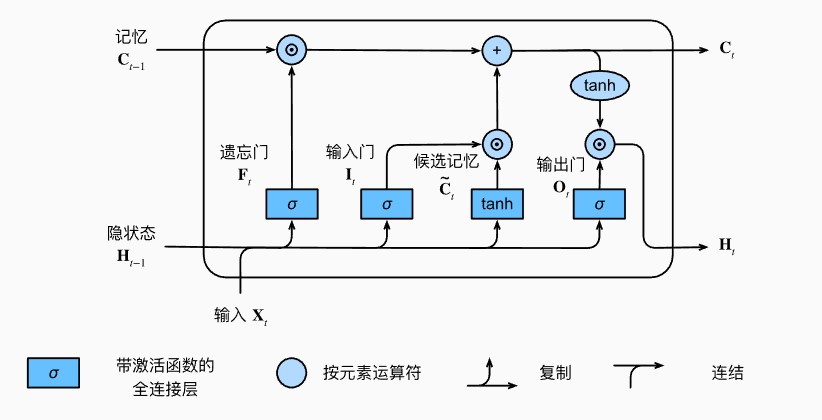
\includegraphics[width=1\textwidth]{LSTM.jpg} %插入图片,[]中设置图片大小,{}中是图片文件名
	\caption{1}
\end{figure}
\end{frame}

\begin{frame}[allowframebreaks]{LSTM}
\begin{itemize}
	\item 首先是定义了输入门,遗忘门,输出门,以及候选记忆单元
	
	\begin{align*}
		&\mathbf{I}_{t} =\sigma(\mathbf{X}_t\mathbf{W}_{xi}+\mathbf{H}_{t-1}\mathbf{W}_{hi}+\mathbf{b}_i), \\
		&\mathbf{F}_{t} =\sigma(\mathbf{X}_t\mathbf{W}_{xf}+\mathbf{H}_{t-1}\mathbf{W}_{hf}+\mathbf{b}_f), \\
		&\mathbf{O}_{t} =\sigma(\mathbf{X}_t\mathbf{W}_{xo}+\mathbf{H}_{t-1}\mathbf{W}_{ho}+\mathbf{b}_o),\\
		&\tilde{\mathbf{C}}_t=\tanh(\mathbf{X}_t\mathbf{W}_{xc}+\mathbf{H}_{t-1}\mathbf{W}_{hc}+\mathbf{b}_c),
	\end{align*}
	其中$\sigma(x)$为$sigmoid$激活函数 ,这些计算实际上和RNN中隐状态的计算比较类似\\
	\item 下面我们定义记忆元
	$$
	\mathbf{C}_t=\mathbf{F}_t\odot\mathbf{C}_{t-1}+\mathbf{I}_t\odot\tilde{\mathbf{C}}_t
	$$
	$\mathbf{F}_t\odot\mathbf{C}_{t-1}$实际上表示了遗忘多少先前的记忆元$\mathbf{C}_{t-1}$,而$\mathbf{I}_t\odot\tilde{\mathbf{C}}_t$ 则代表了当前候选记忆元使用的程度
	\item $LSTM$中隐状态的定义如下:
	$$
	\mathbf{H}_t=\mathbf{O}_t\odot\tanh(\mathbf{C}_t)
	$$
	这样的定义可以保证每个元素均在$[-1,1]$之间,防止梯度爆炸
	\item LSTM层的计算基本是这样,我们取最后一层的隐状态加上Dense输出即可
\end{itemize}\newpage
代码实现如下(仅给出关键代码):
\begin{figure}[H] %H为当前位置,!htb为忽略美学标准,htbp为浮动图形
	\centering %图片居中
	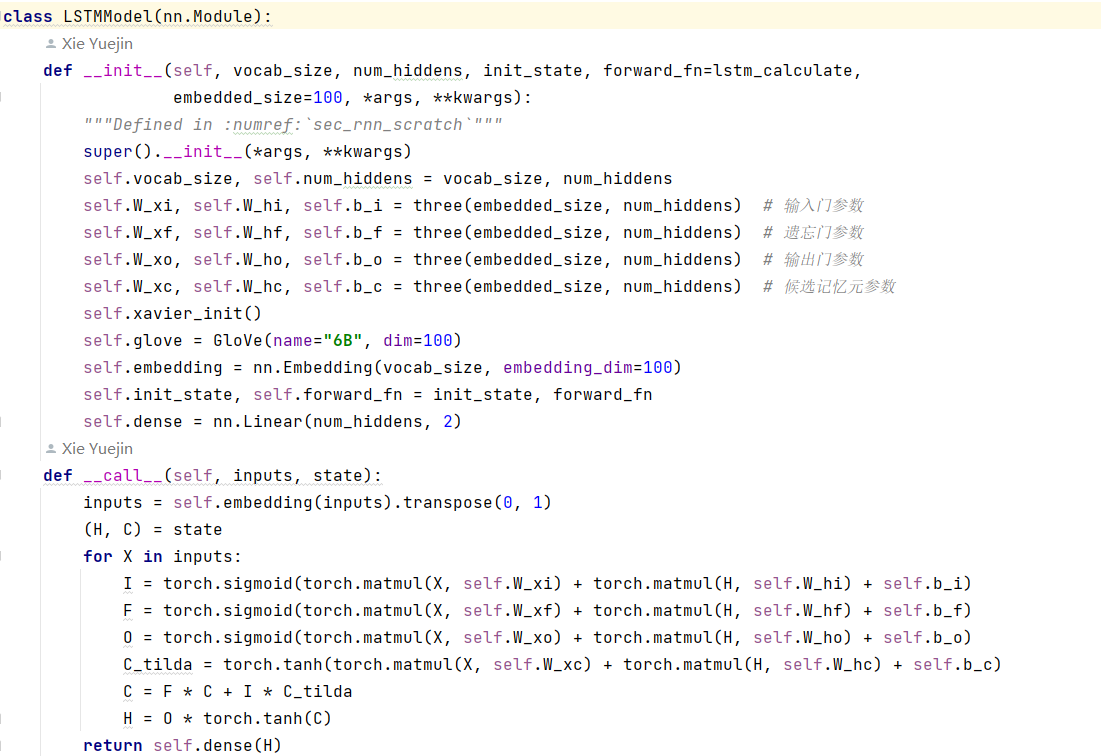
\includegraphics[scale=0.25]{LSTM2.png} %插入图片,[]中设置图片大小,{}中是图片文件名
	\caption{2}
\end{figure}
结果:
\begin{figure}[H] %H为当前位置,!htb为忽略美学标准,htbp为浮动图形
	\centering %图片居中
	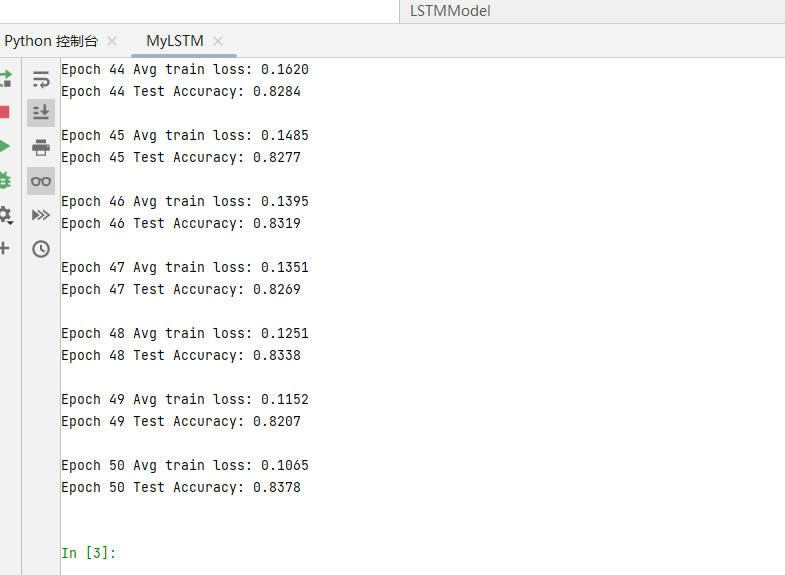
\includegraphics[scale=0.35]{LSTM3.png} %插入图片,[]中设置图片大小,{}中是图片文件名
	\caption{3}
\end{figure}
遇到问题/瑕疵:
\begin{itemize}
	\item 最开始的时候参数矩阵使用了零初始化,导致了梯度消失,损失一直降不下去(改用xavier初始化解决)
	\item 没能实现多层LSTM,以及双向LSTM,使得效果不如框架实现的LSTM
\end{itemize}
\end{frame}

\subsection{TextCNN}
\begin{frame}[allowframebreaks]{TextCNN}
TextCNN的实现总体来说比较轻松,模型图如下:
\begin{figure}[H] %H为当前位置,!htb为忽略美学标准,htbp为浮动图形
	\centering %图片居中
	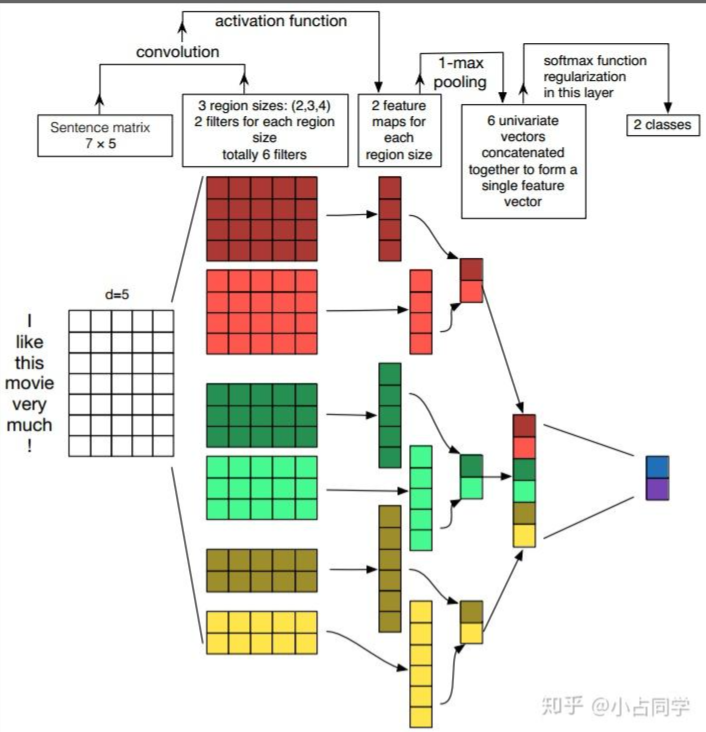
\includegraphics[scale=0.2]{textcnn_model.jpg} %插入图片,[]中设置图片大小,{}中是图片文件名
	\caption{4}
\end{figure}
\begin{itemize}
	\item 第一层:输入层\\
	每个词向量可以是预先在其他语料库中训练好的,也可以作为未知的参数由网络训练得到。预先训练的词嵌入可以利用其他语料库得到更多的先验知识,而由当前网络训练的词向量能够更好地抓住与当前任务相关联的特征。因此,图中的输入层实际采用了双通道的形式,即有两个 $N\times k$ 的输入矩阵,其中一个用预训练好的词嵌入表达,并且在训练过程中不再发生变化;另外一个也由同样的方式初始化,但是会作为参数,随着网络的训练过程发生改变
	\item 第二层:卷积层\\
	把$embedded\_size$当作通道数,对每个通道进行一维卷积,通道求和得到输出,我们可以得到多个输出通道以提升模型的复杂度,让模型提取不同的语义信息
	\item 第三层:池化连接层\\	
	将上一步的输出用最大池化,再进行连接,加上dense层输出二分类的概率即可
\end{itemize}
\end{frame}
\end{document}
